% =====================================================================
% Jev on TGB: an external relevance judge for task-level tool spaces
% TEA template (tea.cls), pdflatex + bibtex
% compiles from this folder or from the project root (Overleaf main document = jev_eval/main.tex)
% =====================================================================
\makeatletter\def\input@path{{jev_eval/}}\makeatother
\documentclass[11pt]{tea}
\graphicspath{{jev_eval/}}

\usepackage{url}
\let\Bbbk\relax
\let\openbox\relax
\usepackage{amsmath}
\usepackage{amssymb}
\usepackage{enumitem}
\usepackage{float}

\newcommand{\JA}{Jev-A}
\newcommand{\JB}{Jev-B}
\newcommand{\JC}{Jev-C}
\newcommand{\tool}[1]{\texttt{#1}}
\newcommand{\task}[1]{\texttt{\detokenize{#1}}}

\title{What Must a Relevance Judge See? Evaluating Jev for Task-Level Tool Selection}

\date{September 2026}

\abstract{
Serving each recurring task with a small tool space instead of the whole registry makes tool-using agents more accurate and cheaper to run. We test whether Jev, the TypeSafe System One model, can decide which tools belong in such a space. On TGB, a compositional benchmark with ten task families and 15 tools, Jev scores every tool with an independent probability in three settings: from the request and tool descriptions for each request, from the same judgments averaged over a task's earlier requests, and from execution traces that show the tool outputs and the executor's answer. From requests alone, Jev often swaps the task's data source for a similar retrieval tool, and since a missing source breaks the whole chain, accuracy falls below serving all tools (60.3\% and 55.2\% against 69.5\%). From execution traces, Jev selects every required tool and reaches 80.7\%, 11.2 points above serving all tools, for a one-time cost of \$0.07. On BFCL multi-turn function calling, where every tool stays callable and the space decides which tools keep full documentation, the order reverses: spaces built from requests raise accuracy from 11.3\% to 16.3--17.3\%, above every baseline (at most 13.8\%), while spaces built from the executor's own traces reach 12.5\%, because those traces are mostly failed attempts. On GTA, where the executor answers few requests under any space, request-based Jev spaces match or exceed the best baseline on the two task types that separate methods.
}

\begin{document}
\maketitle

% ---------------------------------------------------------------------
\section{Introduction}

A tool-using language model is usually served with every tool in its registry \citep{toolformer,gorilla,qin2024toolllm}. For requests that recur within a task, a smaller task-specific space removes distractor tools and shortens every prompt. Building that space means deciding which tools a task needs. Retrieval methods decide from tool descriptions \citep{xiao2024cpack,tool2vec}; trace-based methods decide from what the tools returned and what the model answered \citep{zheng2023judging}.

We ask whether an external relevance model can make this decision. Jev \citep{jevdocs} answers yes/no questions about a shared input with independent probabilities, so one call can score every tool in a registry, and each tool's score stands on its own. It is also cheap (\$0.042 per million input tokens) and fast (about 0.3 seconds per call). We evaluate it on TGB \citep{tgb2026}, BFCL \citep{bfcl}, and GTA \citep{gta} with a fixed executor and find:
\begin{itemize}[leftmargin=*,itemsep=1pt,topsep=2pt]
  \item From the request and tool descriptions, Jev picks the downstream tools but often misses the upstream data source, which breaks the chain.
  \item Averaging these judgments over a task makes them worse, because the same mistake repeats on every request.
  \item From execution traces, Jev selects every required tool and improves on serving all tools by 11.2 points.
  \item On BFCL, request-based spaces beat every baseline and trace-based spaces do not: the executor fails most build conversations, so its traces show the wrong tools.
  \item On GTA, differences are one to three requests; request-based Jev spaces match or exceed the best baseline where methods separate at all.
\end{itemize}

% ---------------------------------------------------------------------
\section{Setup on TGB}

\paragraph{Benchmark.}
TGB has 4,000 text-only requests in ten families of 400 \citep{tgb2026}. Each request is built from a hidden scene (a table, sensor series, calendar, or document corpus) that only the tools can read. Eight families need a chain of two or three tools (Table~\ref{tab:families}); \task{compute_only} and \task{no_tool} are controls. The registry has 15 tools: seven chain tools and eight distractors. Every served tool runs once per request, the chain passes outputs downstream, and the executor sees one line \tool{<Tool>: <output>} per served tool. Accuracy is exact match with the gold answer.

\begin{table}[t]
\centering\small
\caption{TGB families and the budget $K$ shared by all methods.}
\label{tab:families}
\begin{tabular}{@{}llc@{}}
\toprule
Family & Chain & $K$ \\
\midrule
\task{table_total}, \task{table_filter} & \tool{TableQuery} $\to$ \tool{Calculator} & 2 \\
\task{sensor_mean}, \task{sensor_convert} & \tool{SensorAPI} $\to$ \tool{Calculator} & 14 \\
\task{schedule_gap} & \tool{CalendarAPI} $\to$ \tool{Calculator} & 9 \\
\task{doc_two_facts} & \tool{DocRetrieve} $\to$ \tool{Calculator} & 2 \\
\task{translate_fact} & \tool{DocRetrieve} $\to$ \tool{Translate} & 3 \\
\task{fx_settle} & \tool{DocRetrieve} $+$ \tool{ExchangeRate} $\to$ \tool{Calculator} & 3 \\
\task{compute_only} & \tool{Calculator} (optional) & 1 \\
\task{no_tool} & none & 1 \\
\bottomrule
\end{tabular}
\end{table}

\paragraph{Protocol.}
In each family the first 80 requests are used to build spaces and the remaining 320 are evaluated (3,200 in total). The executor is Qwen2.5-7B-Instruct with greedy decoding. Every method keeps the same number of tools per family, a budget $K$ fixed in advance from accuracy on the build requests (Table~\ref{tab:families}). All methods are evaluated in one session on the same requests.

\paragraph{Jev.}
One call scores all 15 tools, with one yes/no question per tool. Tools are described by the first line of their docstring, as in the other baselines; \tool{ExchangeRate} and \tool{Barcode} have no docstring and appear by name. The model version was \texttt{jev-1.13.0}. We test three settings (prompts in Appendix~\ref{app:prompts}):
\begin{itemize}[leftmargin=*,itemsep=1pt,topsep=2pt]
  \item \textbf{\JA{}, per request.} Jev reads an evaluation request and the tool descriptions and is asked whether each tool is needed, including tools whose output feeds another tool. The top $K$ tools serve that request.
  \item \textbf{\JB{}, per task.} The same question on the family's 80 build requests; each tool's scores are averaged, and the top $K$ form a fixed space for the family.
  \item \textbf{\JC{}, per task from traces.} Jev reads a build request, the tool outputs the executor saw, and the executor's answer, and is asked whether the answer relies on each tool's output. Scores are averaged and the top $K$ kept as in \JB{}.
\end{itemize}

\paragraph{Baselines.}
\emph{Keep all} serves the 15 tools. \emph{Random} draws $K$ tools. \emph{Dense} \citep{xiao2024cpack} and \emph{Tool2Vec} \citep{tool2vec} rank tools by embedding similarity to the build requests. \emph{Trace judge} asks the executor itself which tools support its answer on the build traces \citep{zheng2023judging}. \JC{} and Trace judge read the same traces.

% ---------------------------------------------------------------------
\section{Results on TGB}

\begin{table}[t]
\centering\small
\caption{Accuracy averaged over families (3,200 evaluation requests). Coverage: share of requests whose space contains the complete tool chain. Tokens: executor prompt length per request.}
\label{tab:main}
\begin{tabular}{@{}lcccc@{}}
\toprule
Method & Accuracy & vs.\ Keep all & Coverage & Tokens \\
\midrule
Keep all & 69.5 & 0.0 & 1.00 & 271 \\
Random & 23.5 & $-46.0$ & 0.22 & 117 \\
Dense & 24.9 & $-44.6$ & 0.22 & 122 \\
Tool2Vec & 38.1 & $-31.4$ & 0.44 & 123 \\
Trace judge & 67.6 & $-1.9$ & 0.89 & 156 \\
\midrule
\JA{} (per request) & 60.3 & $-9.2$ & 0.73 & 147 \\
\JB{} (per task) & 55.2 & $-14.3$ & 0.67 & 141 \\
\JC{} (per task, traces) & \textbf{80.7} & $+11.2$ & 1.00 & 165 \\
\bottomrule
\end{tabular}
\end{table}

\begin{figure}[t]
\centering
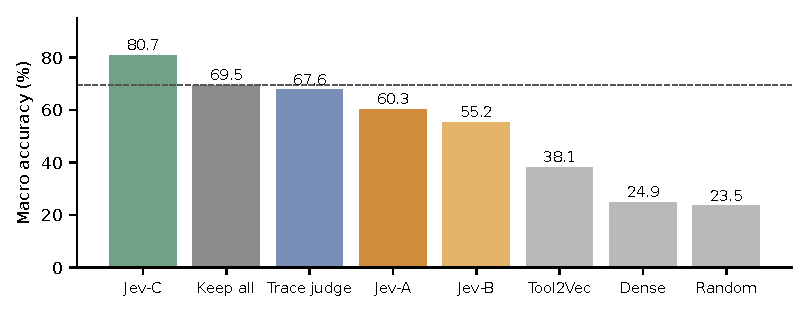
\includegraphics[width=0.8\linewidth]{figs/fig_main.pdf}
\caption{Accuracy of each method at the same budget. Dashed line: Keep all.}
\label{fig:main}
\end{figure}

Table~\ref{tab:main} and Figure~\ref{fig:main} summarize the results. Among the reduced spaces, accuracy follows coverage: \JC{}, which always contains the complete chain, scores above Keep all, and every space that misses the chain on a tenth of the requests or more falls below it. Figure~\ref{fig:family} shows each family.

\subsection{From requests, Jev misses the data source}

\begin{figure}[t]
\centering
\begin{minipage}[c]{0.46\linewidth}
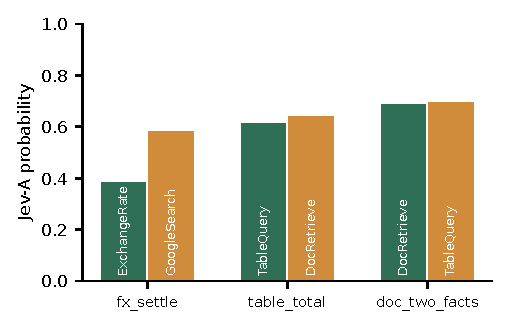
\includegraphics[width=\linewidth]{figs/fig_sources.pdf}
\end{minipage}\hfill
\begin{minipage}[c]{0.5\linewidth}
\captionof{figure}{Mean \JA{} score of the required data source (green) and the tool that replaces it (orange) in the three families where \JA{} fails.}
\label{fig:sources}
\end{minipage}
\end{figure}

\JA{} gives the required tools an average score of 0.77 and the other tools 0.12, and it always selects \tool{Calculator}, the last step of most chains. Its mistakes fall on the first step. In three families it replaces the data source with a similar retrieval tool (Figure~\ref{fig:sources}):
\begin{itemize}[leftmargin=*,itemsep=1pt,topsep=2pt]
  \item \task{fx_settle}: \tool{GoogleSearch} (0.58) replaces \tool{ExchangeRate} (0.39), which has no description, on 270 of 320 requests.
  \item \task{table_total}: \tool{DocRetrieve} (0.64) replaces \tool{TableQuery} (0.61) on 232 requests.
  \item \task{doc_two_facts}: \tool{TableQuery} (0.70) replaces \tool{DocRetrieve} (0.69) on 203 requests.
\end{itemize}
Without its source, the chain cannot compute the answer, and accuracy in these families drops to 0.3\%, 22.5\%, and 28.4\%. In the other families \JA{} is close to Keep all or better.

\subsection{Averaging over a task repeats the mistake}

Jev gives nearly the same score to a tool on every request of a family, so \JA{}'s mistakes are the same mistake repeated. Averaging over the build requests turns these near ties into a fixed wrong choice for the whole family: \JB{} keeps \tool{DocRetrieve} in \task{table_total} and \tool{TableQuery} in \task{doc_two_facts}, and both families fall to 0\%. \JB{} scores 55.2\%, below \JA{} at 60.3\%.

\subsection{From traces, Jev finds every required tool}

\begin{figure}[t]
\centering
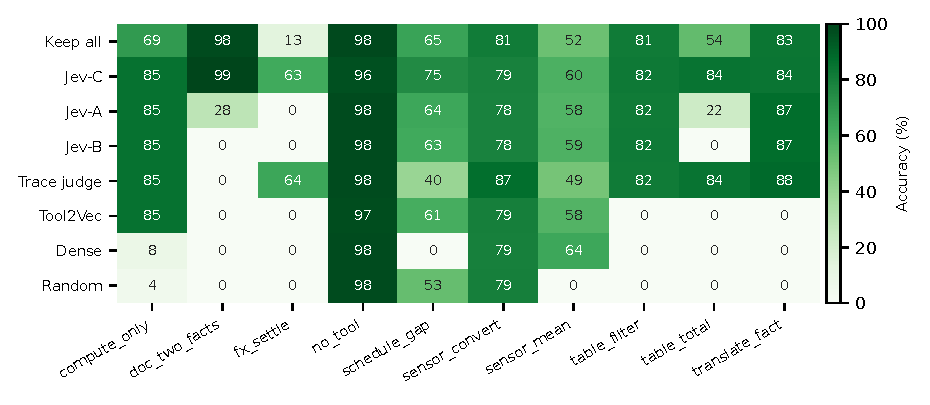
\includegraphics[width=\linewidth]{figs/fig_family.pdf}
\caption{Accuracy (\%) per family on the 320 evaluation requests of each family.}
\label{fig:family}
\end{figure}

With the tool outputs and the answer in view, Jev scores the required tools at 0.78 on average and every other tool at 0.02, and upstream sources score as high as downstream steps. \JC{} contains the complete chain in every family and reaches 80.7\%, recovering \task{doc_two_facts} (99.4\%), \task{fx_settle} (62.8\%), and \task{table_total} (84.1\%). The Trace judge reads the same traces through the executor and reaches 67.6\%.

The remaining errors of \JC{} come from the extra tools that fill the budget in families with a large $K$. Jev gives every non-required tool about the same low score, so the order among distractors carries little information. In \task{sensor_mean} ($K=14$), \JC{} drops \tool{ExchangeRate} and scores 59.7\% (Keep all: 51.9\%); in \task{schedule_gap} ($K=9$) it scores 75.0\% (Keep all: 65.3\%). Ranking distractors by how much they hurt the executor is the part that traces read by Jev leave open.

\subsection{Cost}

\begin{table}[t]
\centering\small
\caption{Cost of the Jev settings at \$0.042 per million input tokens. Latency is per call.}
\label{tab:cost}
\begin{tabular}{@{}lll@{}}
\toprule
Method & Build once & Per evaluation request \\
\midrule
\JA{} & none & 1 call, \$0.00008, 0.31 s \\
\JB{} & 800 calls, \$0.061 & none \\
\JC{} & 800 calls, \$0.073 & none \\
\bottomrule
\end{tabular}
\end{table}

Table~\ref{tab:cost} lists the cost. A Jev task space costs \$0.06 to \$0.07 to build for all ten families and adds nothing per request. \JA{} adds one call and 0.31 seconds to every request, \$0.25 over the 3,200 evaluation requests. Every method at the same budget shortens the executor prompt from 271 tokens to 117 to 165.

% ---------------------------------------------------------------------
\section{BFCL}
\label{sec:bfcl}

\paragraph{Setup.}
We use the 200 records of BFCL v4 \texttt{multi\_turn\_base} \citep{bfcl}, grouped by primary API class (GorillaFileSystem, TradingBot, TravelAPI, VehicleControlAPI), with the first 10 records of each class for building and the other 40 for testing (160 in total). A record's menu holds the functions of its API classes, padded to 30 with functions of other classes. A record succeeds only if the calls across all its turns reach the reference end state, so every tool stays callable: a space is the set of $K$ tools that keep their full documentation, and the other tools keep their signature and one sentence. $K$ is fixed per class from build accuracy (4, 4, 8, and 4). The executor is again Qwen2.5-7B-Instruct, and each method is run three times in one session.

Jev scores the tools of each record's menu as on TGB. \JA{} reads a test record's user turns; \JB{} averages the same scores over the 10 build records of a class. \JC{} reads the executor's build conversations under full documentation (user turns, calls, tool outputs, replies) and is asked whether the assistant relied on each tool it called, to perform an action the user asked for or to feed a later step. A tool that is missing from a build record's menu, or that the executor did not call, counts as 0 in the class average.

\begin{table}[t]
\centering\small
\caption{BFCL, 160 test records (one record is 0.625 points). Every method keeps full documentation for the same $K$ tools per class, except the router, which documents the tools it names for each record. Accuracy is the mean of three runs. Baselines and Jev were run in two sessions on the same server configuration; full documentation was rerun in each (11.0 and 11.3). Recall: share of the reference calls' tools that keep full documentation. Tokens: executor input tokens per record, summed over turns.}
\label{tab:bfcl}
\setlength{\tabcolsep}{4pt}
\begin{tabular}{@{}lcccc@{}}
\toprule
Method & Accuracy & Runs & Recall & Tokens \\
\midrule
Full documentation & 11.0 / 11.3 & {\scriptsize 10.6, 11.3, 11.3 / 11.3, 11.3, 11.3} & 1.00 & 204k / 208k \\
Random & 11.9 & {\scriptsize 11.3, 10.6, 13.8} & 0.17 & 85k \\
BM25 & 12.1 & {\scriptsize 11.9, 12.5, 11.9} & 0.30 & 91k \\
Dense & 12.9 & {\scriptsize 12.5, 13.8, 12.5} & 0.34 & 99k \\
Usage Frequency & 12.7 & {\scriptsize 12.5, 13.1, 12.5} & 0.43 & 97k \\
Tool2Vec & 13.8 & {\scriptsize 13.8, 13.8, 13.8} & 0.28 & 97k \\
LLM as router & 13.5 & {\scriptsize 13.1, 13.8, 13.8} & 0.69 & 84k \\
\midrule
\JA{} (per request) & 16.3 & {\scriptsize 15.6, 16.9, 16.3} & 0.71 & 80k \\
\JB{} (per task) & \textbf{17.3} & {\scriptsize 17.5, 16.9, 17.5} & 0.31 & 90k \\
\JC{} (per task, traces) & 12.5 & {\scriptsize 12.5, 12.5, 12.5} & 0.45 & 93k \\
\bottomrule
\end{tabular}
\end{table}

\paragraph{Results.}
Table~\ref{tab:bfcl} shows the results. \JB{} and \JA{} are the two best methods, 5 to 6 points above full documentation and 2.5 to 3.5 points above the best baselines (Tool2Vec 13.8\%, the router 13.5\%); their lowest runs (16.9\% and 15.6\%) are above the highest run of every baseline (13.8\%). They also cut the executor's input by more than half. The baselines lie between 11.9\% and 13.8\%, and single runs of the same baseline differ by up to 3 points, so their order among themselves is not settled. \JC{} falls in the same range. Most of the Jev gain comes from TradingBot (30.0\% with full documentation, 41.7\% with \JA{}, 39.2\% with \JB{}) and TravelAPI (12.5\%, 15.0\%, 20.0\%).

The trace-based space is weak here because the traces are. The executor solves 20\% of the build records under full documentation, and its conversations are dominated by failed and repeated calls, such as switching to \tool{cp} after a failed \tool{mv} when the user asked to move a file. Jev reads these conversations faithfully, so the tools it credits are the ones the executor used, including the wrong ones, and tools the executor never called receive no credit at all. On TGB, where tool outputs are deterministic and the executor answers most build requests, the same reading recovers every required tool.

Averaging over a class does not hurt on BFCL (\JB{} 17.3\% against \JA{} 16.3\%). Records within a class ask for different subsets of the class's functions, and the class average ranks the commonly needed functions first. Recall of the documented set is also a weak guide here: \JA{} documents more of the reference tools than \JB{} (0.71 against 0.31) at similar accuracy, because an undocumented tool remains callable.

% ---------------------------------------------------------------------
\section{GTA}
\label{sec:gta}

\paragraph{Setup.}
GTA \citep{gta} serves image-based requests with a ReAct agent and an executable tool server. We use three exactly scoreable task types: \task{read_arith} (32 test requests), \task{count_arith} (15), and \task{web_fact} (17, with web search enabled), each split in half into build and test requests. The candidates are the seven tools whose outputs are available (OCR, ImageDescription, Calculator, CountGivenObject, RegionAttributeDescription, TextToBbox, Solver), plus GoogleSearch for \task{web_fact}. Every space keeps $K=2$ tools. Jev reads the request text and the tool descriptions (\JA{}, \JB{}) or the executor's full-menu build trajectories (\JC{}); the images themselves are not shown. The executor is Qwen2.5-7B-Instruct.

\begin{table}[t]
\centering\small
\caption{GTA accuracy (\%) with a two-tool space, all methods in one session. One request is 3.1 points on \task{read_arith}, 6.7 on \task{count_arith}, and 5.9 on \task{web_fact}.}
\label{tab:gta}
\begin{tabular}{@{}lccc@{}}
\toprule
Method & \task{read_arith} & \task{count_arith} & \task{web_fact} \\
\midrule
Keep all & 6.3 & 6.7 & 0.0 \\
No tools & 0.0 & 0.0 & 5.9 \\
Random & 9.4 & 6.7 & 11.8 \\
BM25 & 3.1 & 6.7 & 0.0 \\
Dense & 3.1 & 13.3 & 0.0 \\
Tool2Vec & 3.1 & 6.7 & 0.0 \\
LLM as router & 3.1 & 6.7 & 0.0 \\
TTO & 12.5 & 6.7 & 5.9 \\
Beam Search & 12.5 & 0.0 & 5.9 \\
\midrule
\JA{} (per request) & 12.5 & \textbf{20.0} & 0.0 \\
\JB{} (per task) & 12.5 & 13.3 & 0.0 \\
\JC{} (per task, traces) & 12.5 & 0.0 & 11.8 \\
\bottomrule
\end{tabular}
\end{table}

\paragraph{Results.}
Table~\ref{tab:gta} shows the results. The 7B executor answers few GTA requests under any menu: Keep all solves 2 of 32 \task{read_arith} requests and none of the \task{web_fact} requests, so the methods differ by one to three requests. On \task{read_arith} the three Jev spaces tie with TTO and Beam Search at 4 of 32, above every other method. On \task{count_arith}, \JA{} solves 3 of 15 requests and \JB{} 2, where the best baseline solves 2 and Keep all 1. \JC{} has little to read: the executor calls a tool in 6 of 33 \task{read_arith} and 2 of 15 \task{count_arith} build trajectories, so most tools never appear in a trace, and on \task{count_arith} its space misses the counting tool. On \task{web_fact} no space helps the 7B executor beyond two requests, and a repeated session moves single methods by one request, so the \task{web_fact} column carries no ranking.

% ---------------------------------------------------------------------
\section{Conclusion}

What an external relevance judge should read depends on the quality of the traces. On TGB, tool outputs are reliable and the executor answers most build requests, so the execution trace is the input that matters: from requests Jev confuses similar data sources, and from traces it selects every required tool and improves on serving all tools by 11.2 points. On BFCL, the executor fails most build conversations, so its traces point to the wrong tools, and spaces built from the requests are the ones that help, by 4 to 6 points over serving everything and by 2.5 to 3.5 points over the best baseline. GTA, where the executor solves few requests under any space, points the same way as BFCL. Each setting costs a few cents for a whole benchmark. Next steps are more executors and larger registries, and deciding from the traces themselves when they are good enough to use.

\bibliographystyle{plainnat}
\IfFileExists{jev_eval/refs.bib}{\bibliography{jev_eval/refs}}{\bibliography{refs}}

\beginappendix

\section{Prompts}
\label{app:prompts}

\paragraph{\JA{} and \JB{}.} Input: the request and the 15 tool descriptions. One question per tool \texttt{T}:
\begin{quote}\small\ttfamily
For the user request `request`, would an agent need to call the tool T (described in `tools`) to answer it correctly? Count a tool as needed if its output is required at any step, including intermediate steps whose result feeds another tool. Judge only from the request and the tool descriptions.
\end{quote}

\paragraph{\JC{}.} Input: the request, the tool outputs the executor saw, and the executor's answer. One question per tool \texttt{T}:
\begin{quote}\small\ttfamily
An assistant answered the request `request` after seeing the outputs in `tool\_outputs` and gave the final answer `answer`. Does that answer rely on the output of the tool T? Say yes if the answer uses information that appears in that tool's output, directly or through another tool's output that was computed from it. Do not judge whether the answer is correct and do not answer the request yourself.
\end{quote}

\section{Task spaces}

\begin{table}[H]
\centering\small
\caption{Jev task spaces in the families where \JB{} and \JC{} differ. Chain tools in bold; for $K=14$ the dropped tool is listed.}
\setlength{\tabcolsep}{4pt}
\begin{tabular}{@{}lp{4.8cm}p{4.8cm}@{}}
\toprule
Family & \JB{} & \JC{} \\
\midrule
\task{doc_two_facts} & \textbf{Calculator}, TableQuery & \textbf{DocRetrieve}, \textbf{Calculator} \\
\task{fx_settle} & \textbf{Calculator}, \textbf{DocRetrieve}, GoogleSearch & \textbf{DocRetrieve}, \textbf{Calculator}, \textbf{ExchangeRate} \\
\task{table_total} & \textbf{Calculator}, DocRetrieve & \textbf{Calculator}, \textbf{TableQuery} \\
\task{translate_fact} & \textbf{DocRetrieve}, \textbf{Translate}, Calculator & \textbf{Translate}, \textbf{DocRetrieve}, Barcode \\
\task{sensor_mean} & all but CurrencyConvert & all but ExchangeRate \\
\task{sensor_convert} & all but DurationCalc & all but CurrencyConvert \\
\task{no_tool} & Calculator & Barcode \\
\bottomrule
\end{tabular}
\end{table}

\end{document}
